\chapter{Graphs}

This chapter will provide relevant background material in the theory of graphs.

If \(X\) is a set, and \(k\in\N\) is a natural number (including zero), then \(\binom Xk=\setb{A\sbset X}{\card A=k}\) is the set of unordered \(k\)-tuples of elements of \(X\).

\section{Definition and Examples}
    A graph is an ordered pair \(G=(V,E)\) where \(V\) is a finite set, and \(E\sbset\binom V2\) is a set of unordered pairs of elements of \(V\).  The elements of \(V=V(G)\) are called \dfn{vertices}, and the  elements of \(E=E(G)\) are called \dfn{edges}. Note that either \(V\) or \(E\) is allowed to be empty.  If \(V=\mt\), then \(E=\mt\), and \(G\) is called the \dfn{empty graph}.  If \(e=\seta{x,y}\in E\) and no confusion may arise, the edge \(e\) may be denoted \(e=xy=yx=\seta{x,y}\).  Two vertices \(v,w\in V\) are called \dfn{neighbors}, or \dfn{adjacent} if \(vw\in E\).  The \dfn{neighborhood} of a vertex \(v\) is the set \(N(v)=\setb{w\in V}{vw\in E}\) of all neighbors of \(v\).  The \dfn{degree} of a vertex \(v\) is the number of edges on which \(v\) lies, that is, \(\deg v=\card{\setb{e\in E}{v\in e}}=\card{N(v)}\).

    Two graphs \(G=(V,E)\) and \(H=(W,F)\) are said to be \dfn{isomorphic} if a bijection \(\phi\colon V\to W\) exists with the additional property: \(xy\in E\) if and only if \(\phi(x)\phi(y)\in F\).  If \(G\) and \(H\) are isomorphic, no distinction will be made between them.  It is often useful to draw a graph by depicting its vertices as points in the plane, and its edges by continuous curves between vertices.
        \begin{Examples}\(\phantom.\)
            \begin{enumerate}
                \item   A \dfn{discrete} graph on \(n\) vertices is a graph isomorphic to \(D_n=(\brac n,\mt)\).
                \item   A \dfn{cycle} of \dfn{length} \(n\ge3\) is a graph isomorphic to \(C_n\) where \(V(C_n)=\brac n\) and
                        \[
                            E(C_n)=\setb{ij}{i-j\equiv1\pmod n}.
                        \]
                        \begin{center}
                            \begin{figure}[h!bt]
                                \includegraphics[page=13, width=.8\textwidth]{pictures.pdf}
                                \caption{Several cycle graphs.}
                            \end{figure}
                        \end{center}
                \item   A graph is \dfn{complete} if \(E=\binom V2\).  If \(\card V=n\), then \(G\) is denoted \(K_n\).
                        \begin{center}
                            \begin{figure}[h!bt]
                                \includegraphics[page=8, width=.8\textwidth]{pictures.pdf}
                                \caption{Several complete graphs.}
                            \end{figure}
                        \end{center}
                \item   A graph \(G\) is said to be \dfn{bipartite} if \(V(G)=V_1\cup V_2\) with \(V_1\ne\mt\ne V_2\) and \(V_1\cap V_2=\mt\) such that \(E(G)\cap\binom{V_1}2=E(G)\cap\binom{V_2}2=\mt\).  If \(G\) is a bipartite graph satisfying
                        \[
                            E(G)=\setb{xy\in\binom V2}{x\in V_1\text{ and }y\in V_2},
                        \]
                    then \(G\) is \dfn{complete bipartite}, and is denoted \(K_{n,m}\) where \(\card{V_1}=n\) and \(\card{V_2}=m\).  Note that a complete bipartite graph must have at least one edge.
                        \begin{center}
                            \begin{figure}[h!bt]
                                \includegraphics[page=9, width=.8\textwidth]{pictures.pdf}
                                \caption{Several bipartite graphs.  The first vertex set is colored white, and the second black.}
                            \end{figure}
                        \end{center}
                \item   More generally, a graph is \dfn{\(n\)-partite} if its vertex set can be written  \(V(G)=\bigcup_{i\in\brac n}V_i\) such that:
                        \begin{enumerate}
                            \item   \(V_i\ne\mt\) for all \(i\in\brac n\);
                            \item   \(V_i\cap V_j=\mt\) for \(i\ne j\); and
                            \item   \(E(G)\cap\binom{V_i}2=\mt\) for each \(i\in\brac n\).
                        \end{enumerate}
                    In this case, \(V(G)\) will be written as \(\bigsqcup_{i\in\brac n}V_i\) and the sets \(V_i\) are called \dfn{color classes}.

                    If, additionally, \(E(G)=\setb{xy\in\binom V2}{\seta{x,y}\not\sbset V_i\text{ for each }i\in\brac n}\), then \(G\) is called \dfn{complete \(n\)-partite}, and denoted \(K_{m_1,m_2\dc m_n}\) where \(\card{V_i}=m_i\) for each \(i\in\brac n\).  Note that for any permutation \(\sigma\) of \(\brac n\) the graphs \(K_{m_1,m_2\dc m_n}\) and \(K_{m_{\sigma1},m_{\sigma2}\dc m_{\sigma n}}\) are isomorphic.  Hence complete \(n\)-partite graphs will be assumed to satisfy \(m_1\le m_2\le\dotsb\le m_n\).
                        \begin{center}
                            \begin{figure}[h!bt]
                                \includegraphics[page=10, width=.8\textwidth]{pictures.pdf}
                                \caption{Several complete $3$-partite graphs.}
                            \end{figure}
                        \end{center}
            \end{enumerate}
        \end{Examples}

    If \(G\) and \(H\) are graphs, then their \dfn{join} is the graph \(G\join H\) that is defined by
        \begin{gather*}
            V(G\join H)
                =  V(G)\cup V(H)\\
            E(G\join H)
                =  E(G)\cup E(H)\cup \setb{gh}{g\in V(G)\text{ and }h\in V(H)}.
        \end{gather*}
    If \(r,s\) are positive integers, then \(K_{r,s}=D_r\join D_s\), and more generally,
        \[
            K_{r_1,r_2\dc,r_t}
                =   D_{r_1}\join D_{r_2}\join\dotsb\join D_{r_t}.
        \]

\section{Subgraphs and Minors}
    If \(G=(V,E)\) is a graph, then a \dfn{subgraph} \(H\) of \(G\) is a graph of the form \(H=(W,F)\) with \(W\sbset V\), and \(F\sbset E\cap\binom W2\).  If, additionally, for all \(xy\in E(G)\) the containment \(\seta{x,y}\sbset V(H)\) implies the containment \(xy\in E(H)\), that is, \(F=E\cap\binom W2\), then \(H\) is said to be an \dfn{induced subgraph} of \(G\).  When working with graphs, subgraphs are not generally sufficient for dealing with statements of theorems; the idea of a minor of a graph is also needed:
        \begin{Definitions}
             Let \(G=(V,E)\) be a graph, and \(W\sbset V\).
                \begin{enumerate}
                    \item   The \dfn{restriction} of \(G\) to \(W\), denoted by \(\rest GW\), is the graph defined by \(V(\rest GW)=W\), and \(E(\rest GW)=E\cap\binom W2\).
                    \item   The \dfn{deletion} of \(W\), denoted \(G\setminus W\), is the restriction of \(G\) to \(V\setminus W\), that is \(\rest G{V\setminus W}\).
                    \item   If \(xy=e\in E\), then the \dfn{contraction} of \(e\), denoted by \(G/e\), is the graph defined by \(V(G/e)=(V\setminus\seta{x,y})\cup\seta{\tilde e}\) and
                            \[
                                E(G/e)
                                    =
                                    E(\rest G{V\setminus\seta{x,y}})
                                        \cup
                                        \setb{\wt ez}{xz\in E\text{ or } yz\in E\text{ and }z\notin\seta{x,y}}
                            \]
                    \item   If \(F\sbset E\), then the \dfn{deletion} of \(F\), denoted \(G\setminus F\), is the graph with \(V(G\setminus F)=V\) and \(E(G\setminus F)=E\setminus F\).
                    \item   A graph \(H\) is a \dfn{minor} of a graph \(G\) if \(H\) is isomorphic to a graph that is obtainable from \(G\) through a sequence of deletions and contractions.
                \end{enumerate}
            \begin{center}
                \begin{figure}[h!bt]
                    \includegraphics[page=11, width=.9\textwidth]{pictures.pdf}
                    \caption{Examples of some minors of a graph $G$.}
                \end{figure}
            \end{center}
        \end{Definitions}
    The word deletion is defined in two different ways above; however no confusion should arise since one definition was in regards to a set of vertices, whereas the other refers to a set of edges.

    \begin{Example}\label{Ex:KThrThrMnr}
        The graph \(K_{3,3}\) has a \(K_4\) minor.  Let \(V(K_{3,3})=\seta{a_1,a_2,a_3}\sqcup\seta{b_1,b_2,b_3}\).  First contract the edge \(a_2b_2\), then contract the edge \(a_3b_3\).  See Figure \ref{Fig:KThrThrMnr}.

            \begin{figure}[ht]
                \centering
                    \includegraphics[width=.8\textwidth, page=28]{pictures.pdf}
                \caption{\protect$K_{3,3}\protect$ has a \protect$K_4\protect$ minor.\label{Fig:KThrThrMnr}}
            \end{figure}
    \end{Example}

    If \(F=\{e_1,e_2\dc e_n\}\sbset E(G)\), then it can be shown that \((\dotsb((G/e_1)/e_2)\dotsb)/e_n\) is isomorphic to \((\dotsb((G/e_{\sigma1})/e_{\sigma2})\dotsb)/e_{\sigma n}\) for any permutation \(\sigma\) of \(\brac n\).  For details see \cite{Diestel}.  This graph is denoted \(G/F\).

\section{Planarity and Connectivity}
    When drawing a graph \(G\) in the plane, a natural question to ask is, ``Is it possible to draw \(G\) such that no two edges intersect unless they share a vertex, and in that case only at the shared vertex?'' If the answer to this question is yes, then the graph is called \dfn{planar}. The following gives a characterization of planarity that avoids topology.  For a proof, see \cite{Wagner} or \cite{Diestel}.

    \begin{Theorem}[Wagner 1937]\label{Thm:Wagner}
        A graph \(G\) is planar if and only if \(G\) has no minor isomorphic to either \(K_5\) or \(K_{3,3}\).
    \end{Theorem}

    As mentioned above, the statement of Theorem \ref{Thm:Wagner} must be in terms of minors; the Peterson graph \(P\) (Figure \ref{Fig:Peterson}) has neither a \(K_5\) nor \(K_{3,3}\) subgraph; however, it does contain each as a minor.  The graph \(K_5\) can be realized by contracting each of the edges \(v_iw_i\) for \(i\in\brac5\), while \(K_{3,3}\) can be realized as \(\left(P\setminus\seta{w_2w_3, v_5w_5}\right)/\seta{w_4w_5, v_2v_5, w_1w_2, v_3w_3}\).

    \begin{figure}[ht]
        \centering
            \includegraphics[width=.3\textwidth, page=12]{pictures.pdf}
        \caption{The Peterson graph.\label{Fig:Peterson}}
    \end{figure}

    Whenever planarity is needed, the above conditions will be checked.  Thus the above definition will be treated as the definition of planarity, and the previous discussion will be reserved for geometric intuition.

    A graph \(G\) is said to be \dfn{connected} if either \(\card V=1\), or for any pair \(x,y\in V\) there exists a sequence of vertices \(x=x_1, x_2\dc x_{r+1}=y\) such that \(x_ix_{i+1}\in E\) for \(i\in\brac r\).  If, additionally, \(x_i\neq x_j\) for \(i\neq j\), then \(x_1,x_2\dc x_{r+1}\) is called a \dfn{path} from \(x\) to \(y\) of \dfn{length} \(r\) with \dfn{endpoints} \(x\) and \(y\).  If \(d\in\N\), then a graph \(G\) is said to be \dfn{\(d\)-connected} if \(\card V>d\), and for \(W\sbset V\) with \(\card W<d\) the graph \(G\setminus W\) is connected.  Every non-empty graph is \(0\)-connected, and the \(1\)-connected graphs are exactly the connected graphs with at least two vertices.

    Two paths \(x_1,x_2\dc x_i\) and \(y_1,y_2\dc y_j\) are said to be \dfn{disjoint} if the only intersections of the paths are at endpoints of each.  The following theorem (equivalent to Menger's Theorem, but first stated in this form by Whitney) gives a characterization of \(d\)-connectedness in terms of disjoint paths. For a proof, see either \cite{Whitney} or \cite{Diestel}.
        \begin{Theorem}[Whitney 1932]
            A graph \(G\) is \(d\)-connected if and only if for all \(a,b\in V\) with \(a\neq b\) there exist \(d\) pairwise disjoint paths from \(a\) to \(b\).
        \end{Theorem}

    \begin{Example}\label{Ex:X3conn}
        The graph \(K_{2,2,2}\) is \(4\)-connected.  Let \(V(K_{2,2,2})=\seta{a_{1,1},a_{2,1},a_{3,1},a_{1,2},a_{2,2},a_{3,2}}\), and \(E(K_{2,2,2})=\setb{a_{i,j}a_{k,l}}{i\ne k}\). Then a pair of vertices \(a_{i,j}a_{k,l}\) is either adjacent, or not.  In the latter case assume, without loss of generality, that \(i=j=k=1\), and \(l=2\).  The following are four pairwise disjoint paths from \(a_{1,1}\) to \(a_{1,2}\):
            \begin{align*}
                &a_{1,1}, a_{2,1}, a_{1,2}&
                        &a_{1,1}, a_{2,2}, a_{1,2}&\\
                &a_{1,1}, a_{3,1}, a_{1,2}&
                        &a_{1,1}, a_{3,2}, a_{1,2}&
            \end{align*}
        If, on the other hand, \(i\ne k\), then assume again that \(i=j=1\), and without loss of generality, assume \(k=3\) and \(l=2\).  Then the following are four pairwise disjoint paths from \(a_{1,1}\) to \(a_{3,2}\):
            \begin{align*}
                &a_{1,1}, a_{3,2}&
                        &a_{1,1}, a_{2,1}, a_{3,2}&\\
                &a_{1,1}, a_{2,2}, a_{3,2}&
                        &a_{1,1}, a_{3,1}, a_{1,2}, a_{3,2}.&
            \end{align*}

            \begin{figure}[ht]
                \centering
                    \includegraphics[width=.5\textwidth, page=21]{pictures.pdf}
                \caption{\protect$K_{2,2,2}\protect$ is \protect$4\protect$-connected.\label{Fig:X3conn}}
            \end{figure}
    \end{Example}


    If \(G\) is a graph, then the \dfn{connectivity}\footnote{This is usually called the \dfn{edge-connectivity} of the graph.  However no other types of connectivity will be considered, so no confusion should arise.} of \(G\) is \(\conn G=\max\setb{k}{G\text{ is }k\text{-connected}}\), and the \dfn{Hadwiger number} of \(G\) is \(\had G=\max\setb{n}{K_n\text{ is a minor of }G}\).
\section{Graphs of Polytopes}{\label{Sec:GraphsOfPolytopes}}
    If \(P\) is a polytope, then the \dfn{graph} of \(P\), denoted \(\gr P\), is the graph with \(V(\gr P)=\vrt P\), and \(E(\gr P)=\setb{\ve x\ve y\in\binom{\vrt P}2}{\conv\seta{\ve x,\ve y}\text{ is an edge of }P}\).   The following theorem is a special case of a more general theorem proven in \cite{GrunBook}.

    \begin{Theorem}[Gr\"unbaum]\label{Thm:CompleteMinor}
        If \(P\) is a \(d\)-polytope, then \(\gr P\) has a \(K_{d+1}\) minor.
    \end{Theorem}
    \begin{proof}
        If \(\dim P=-1\), then \(\gr P\) is empty, i.e., \(K_0\).  If \(\dim P=0\), then \(\gr P\) has one vertex and no edges , i.e., \(K_1\).  If \(\dim P=1\), then \(\gr P\) has two vertices and one edge , i.e., \(K_2\). The proof now proceeds by induction on \(d\).

        Suppose for some \(d\ge2\) that \(K_d\) is a minor of the graph of every \((d-1)\)-polytope.  Let \(P\) be a \(d\)-polytope and \(F\) be a facet of \(P\).  By the induction hypothesis, \(F\) has a \(K_d\) minor.  Fix one such minor.  Each vertex in this minor comes from a vertex of \(F\).  Let \(\seta{\ve v_1, \ve v_2\dc\ve v_n}\) be a set of vertices of \(F\) such that each \(\ve v_i\) corresponds to a different vertex in the complete minor.  Since \(\dim P\ge 2\), each \(\ve v_i\) is on an edge with another vertex \(\ve w_i\in\vrt P\setminus\vrt F\) (it is possible that \(\seta{\ve w_1, \ve w_2\dc\ve w_n}\) has cardinality less than \(n\)).  Now, in \(\gr P\) first perform a sequence of deletions and contractions to obtain the chosen \(K_d\) minor of \(\gr F\), and then contract all edges in this new graph that are not incident to any vertex in the copy of \(K_d\).  This leaves the \(K_d\) minor and one other vertex.  This vertex is adjacent to each vertex in the \(K_d\) minor.  Thus a \(K_{d+1}\) minor of \(\gr P\) has been constructed.
    \end{proof}

    \begin{Example}
        Let \(P\) be the triangular prism whose graph is shown in Figure \ref{Fig:CompleteMinor} and \(F\) be the facet \(\conv\seta{v_1,v_2,v_3,v_4}\).  Note that \(F\) has a \(K_3\) minor that is obtained by contracting \(v_3v_4\).  The first arrow indicates forming that \(K_3\) minor by contracting the edge \(v_3v_4\) in \(\gr P\).  Now the only edge with no vertices corresponding to any of \(v_1,v_2,v_3\) is \(e\).  The second arrow indicates the contraction of \(e\).  This results in a \(K_4\) minor.

            \begin{figure}[ht]
                \centering
                    \includegraphics[width=.8\textwidth, page=27]{pictures.pdf}
                \caption{Example of Theorem \ref{Thm:CompleteMinor}.\label{Fig:CompleteMinor}}
            \end{figure}
    \end{Example}

    The following theorem about the connectivity of graphs of \(d\)-polytopes was proved in \cite{Balinski} using linear programming techniques.

    \begin{Theorem}[Balinski 1961]\label{Thm:ConnectivityOfGraph}
        If \(P\) is a \(d\)-polytope, then \(\gr P\) is \(d\)-connected.
    \end{Theorem}

    The converse is not true.  The \(3\)-dimensional crosspolytope has graph \(K_{2,2,2}\), and is \(4\)-connected (see Example \ref{Ex:X3conn}).  It is also planar, and therefore does not contain a \(K_5\) minor.  Thus it is not the graph of any \(4\)-dimensional polytope.

    Theorems \ref{Thm:CompleteMinor} and \ref{Thm:ConnectivityOfGraph} imply:
    \begin{Corollary}
        If \(G\) is the graph of a \(d\)-polytope, then
            \[
                d\le\min\seta{\had G-1, \conn G}.
            \]
    \end{Corollary}

    This bound will be important in Chapter \ref{chap:CompMulti}.  Notice that these two numbers are, in general, incomparable.  Let \(F\) be any facet of \(\cyc64\), and \(P=K(\cyc64;F)\).  Then \(\had P=6\), and \(\conn P=4\).  On the other hand, if \(R\) is the regular icosahedron, then \(\had R=4\), and \(\conn R=5\).
    
    The following theorem can be found in \cite{ZieglerBook}, albeit without a proof.

\begin{Theorem}\label{Thm:Induced}
        If \(F\) is a face of a polytope \(P\), then \(\gr F\) is an induced subgraph of \(\gr P\).
    \end{Theorem}
    \begin{proof}
        If \(F=\mt\), then \(\gr F\) is the empty graph which is an induced subgraph of every graph.  If \(F=P\), then \(\gr F=\gr P\) and any graph is an induced subgraph of itself.

        Thus, suppose \(F\) is a proper face of \(P\), and write
            \[
                \mt
                    \ne
                    \vrt F
                        =
                        \seta{\ve v_1,\ve v_2\dc\ve v_n}
                            \varsubsetneq
                            \vrt P
            \]
        If \(\ve v_i\ve v_j\in E(\gr P)\), then there is a hyperplane \(H\) such that \(P\cap H=\conv\seta{\ve v_i,\ve v_j}\) and \(P\sbset H^+\).  Hence,
            \begin{align*}
                \conv\seta{\ve v_i,\ve v_j}
                    &=  \conv\seta{\ve v_i,\ve v_j}\cap H\\
                        &\sbset
                        \conv\seta{\ve v_1,\ve v_2\dc\ve v_n}\cap H\\
                            &=
                            F\cap H\\
                                &\sbset
                                P\cap H\\
                                    &=
                                    \conv\seta{\ve v_i,\ve v_j}
            \end{align*}
        where the first equality follows since \(\conv\seta{\ve v_i,\ve v_j}\sbset H\).  Therefore equality holds throughout.  Hence \(F\cap H=\conv\seta{\ve v_i,\ve v_j}\), whence \(H\) is a supporting hyperplane of the face \(\conv\seta{\ve v_i,\ve v_j}\) of \(F\).  Thence \(\ve v_i\ve v_j\in E(\gr F)\).
    \end{proof}

    If \(G\) is a graph, and \(P\) a \(d\)-polytope with \(\gr P=G\), then \(G\) is said to be \dfn{\(d\)-realizable}.  A major open problem in the theory of polytopes is to give a complete characterization of the graphs that are \(d\)-realizable for a fixed \(d\).  One can similarly ask, for a fixed graph \(G\), for which \(d\) is \(G\) \(d\)-realizable?  The cyclic polytopes provide examples of graphs that are \(d\)-realizable for multiple values of \(d\).  Gr\"unbaum asks in \cite{GrunBook} a question, that in the case of graphs becomes: if \(G\) is both \(d\)-realizable and \(d'\)-realizable, then is it \(d''\)-realizable for every \(d''\) between \(d\) and \(d'\)?

    The following theorem gives a complete characterization of the graphs that are \(3\)-realizable.  Proofs can be found in \cite{Steinitz:Paper}, \cite{Steinitz}, \cite{GrunBook}, or \cite{ZieglerBook}.
    \begin{Theorem}[Steinitz 1922]\label{Thm:Steinitz}
        A graph \(G\) is the graph of a \(3\)-polytope if and only if \(G\) is both planar and \(3\)-connected.
    \end{Theorem}

    \begin{Corollary}
        If \(G\) is a \(3\)-connected graph, then \(G\) has a \(K_4\) minor.
    \end{Corollary}
    \begin{proof}
        If \(G\) is planar, then it is \(3\)-realizable, and thus by Theorem \ref{Thm:CompleteMinor} it has a \(K_4\) minor.

        On the other hand, if \(G\) is not planar, then it has either a \(K_{3,3}\) or a \(K_5\) minor.  In the former case, Example \ref{Ex:KThrThrMnr} shows that \(G\) has a \(K_4\) minor.  In the latter, \(K_m\) is a minor of \(K_n\) if and only if \(m\le n\), so that \(K_4\) is a minor of \(K_5\).
    \end{proof}

    A complete characterization of the graphs of polytopes with dimension less than or equal to three can be found in Table \ref{Table:GraphsOfPolytopes}.

        \begin{table}[h!tb]
        \begin{center}\caption{Characterizations of graphs of $d$-polytopes for $d\le3$.}\label{Table:GraphsOfPolytopes}\doublespacing
            \begin{tabular}{c|p{.75\textwidth}}
                Dimension   &   Characterization of Graph\\\hline
                \(-1\)      &   The only \((-1)\)-dimensional polytope is the empty polytope, and it has the empty graph.\\
                \(0\)       &   The only combinatorial type of \(0\)-dimensional polytope is a single vertex.  This has graph \(K_1\).\\
                \(1\)       &   The only combinatorial type of \(1\)-dimensional polytope is a closed line segment.  This has graph \(K_2\).\\
                \(2\)       &   The \(2\)-polytopes are exactly the convex \(n\)-gons lying in a plane, and therefore have graphs that are cycle graphs.  Further, every cycle graph is the graph of a \(2\)-polytope.\\
                \(3\)       &   Theorem \ref{Thm:Steinitz} gives a complete characterization of the graphs of \(3\)-polytopes as the planar \(3\)-connected graphs.
            \end{tabular}
        \end{center}
        \end{table} 